% =====================================================================
%  Tables and figures for the MDPI Computers manuscript
%  "Text Segmentation for Indonesian and Its Regional Languages"
%
%  Paste each block into the MDPI LaTeX template (mdpi.cls), which already
%  loads booktabs, tabularx, float ([H]) and graphicx. Add to the preamble:
%
%    \usepackage{tikz}
%    \usetikzlibrary{arrows.meta,positioning,fit}
%    \usepackage{pgfplots}
%    \pgfplotsset{compat=1.18}
%
%  Numbers come from the runs of 16 November 2026 (heading echo removed
%  unless stated). Cells still running or not yet run are marked:
%    \pend = run in progress, \tbd = needs GPU / API run, see notes.
%  Search for \pend and \tbd before submission; none may remain.
% =====================================================================

\providecommand{\pend}{\textit{running}}
\providecommand{\tbd}{\textit{TBD}}

% ---------------------------------------------------------------------
%  Figure 1. Benchmark pipeline (TikZ, no image file needed)
% ---------------------------------------------------------------------
\begin{figure}[H]
\centering
\begin{tikzpicture}[
  font=\scriptsize,
  box/.style={draw, rounded corners=3pt, align=left, inner sep=4pt,
              text width=2.75cm, minimum height=1.75cm, execute at begin node=\raggedright},
  key/.style={box, very thick, fill=blue!7},
  arr/.style={-{Stealth[length=2mm]}, semithick},
  node distance=1.0cm and 0.35cm]
  \node[box] (src) {\textbf{Sources}\\Wikipedia dumps\\Regional corpora};
  \node[box, right=of src] (ext) {\textbf{Extraction}\\WikiExtractor (HTML)\\patched for nested\\lists and link markup};
  \node[key, right=of ext] (ds) {\textbf{Dataset}\\Drop boilerplate\\Split sentences\\\textbf{Remove heading echo}\\Filter documents};
  \node[box, right=of ds] (seg) {\textbf{Segmenters}\\Classical\\Topic models\\Sentence encoders\\LLM prompting};
  \node[box, below=of seg] (ev) {\textbf{Evaluation}\\$P_k$ and WindowDiff\\Oracle-$k$ and $k$-free\\Runtime and cost};
  \node[box, below=of ds] (sum) {\textbf{Summarization}\\Sets A--D: unsegmented,\\fixed-size, automatic\\and gold segments};
  \node[box, below=of ext] (hum) {\textbf{Human evaluation}\\Native speakers rank\\the four summaries;\\Friedman, Nemenyi};
  \draw[arr] (src) -- (ext);
  \draw[arr] (ext) -- (ds);
  \draw[arr] (ds) -- (seg);
  \draw[arr] (seg) -- (ev);
  \draw[arr] ([xshift=-8mm]seg.south) -- ++(0,-0.45) -| node[pos=0.25, below] {best segmentation} (sum.north);
  \draw[arr] (sum) -- (hum);
\end{tikzpicture}
\caption{Benchmark pipeline. Corpora are extracted and turned into segmentation datasets with the heading echo removed. Every segmenter is scored with $P_k$ and WindowDiff, and the best segmentation feeds the summarization study.\label{fig:pipeline}}
\end{figure}

% ---------------------------------------------------------------------
%  Table 1. Corpus statistics
% ---------------------------------------------------------------------
\begin{table}[H]
\caption{Corpus statistics. Usable documents have at least three section headings, three boundaries and 11 sentences after boilerplate sections are dropped. Sentence and segment counts are for the setting with the heading echo removed.\label{tab:corpus}}
\newcolumntype{C}{>{\centering\arraybackslash}X}
\begin{tabularx}{\textwidth}{lCCCCC}
\toprule
\textbf{Language} & \textbf{Articles} & \textbf{Usable, Cue Kept} & \textbf{Usable, Cue Removed} & \textbf{Sentences per Doc} & \textbf{Segments per Doc}\\
\midrule
Indonesian (id) & 1,356,980 & 60,798 & 49,177 & 63.7 & 6.9\\
Javanese (jv)   & 76,082    & 2,361  & 1,865  & 45.8 & 5.8\\
Sundanese (su)  & 63,237    & 2,065  & 1,701  & 59.3 & 6.9\\
% Minangkabau (min) & \tbd & \tbd & \tbd & \tbd & \tbd\\
% Banjar (bjn)      & \tbd & \tbd & \tbd & \tbd & \tbd\\
% Acehnese (ace)    & \tbd & \tbd & \tbd & \tbd & \tbd\\
\bottomrule
\end{tabularx}
\end{table}

% ---------------------------------------------------------------------
%  Table 2. Segmentation methods
% ---------------------------------------------------------------------
\begin{table}[H]
\caption{Segmentation methods. All are unsupervised and use a window of three sentences. Except TextTiling and BayesSeg-MD, they receive the gold number of segments $k$ (oracle-$k$ setting).\label{tab:methods}}
\newcolumntype{L}{>{\raggedright\arraybackslash}X}
\begin{tabularx}{\textwidth}{lLL}
\toprule
\textbf{Group} & \textbf{Methods} & \textbf{Representation}\\
\midrule
Classical   & TextTiling~\cite{hearst1997}, C99~\cite{choi2000}, CVS~\cite{alemi2015} & Word overlap, TF--IDF\\
Topic model & TopicTiling~\cite{riedl2012}, BayesSeg~\cite{du2013}, BayesSeg-MD~\cite{mota2016}, BeamSeg~\cite{mota2019}, BERTopic~\cite{grootendorst2022} & LDA (100 topics), Dirichlet--multinomial segments, topic clusters\\
Encoder     & Congen-IndoBERT, NusaBERT, LaBSE, Qwen3-Embedding-0.6B & Mean-pooled sentence vectors\\
LLM         & \tbd{} (open-weight and proprietary) & Numbered sentences in, boundary indices out (JSON)\\
\bottomrule
\end{tabularx}
\end{table}

% ---------------------------------------------------------------------
%  Table 3. Reproduction of the conference results (cue kept)
% ---------------------------------------------------------------------
\begin{table}[H]
\caption{Reproduction of the conference results on 60,798 Indonesian documents with the heading cue kept.\label{tab:repro}}
\newcolumntype{C}{>{\centering\arraybackslash}X}
\begin{tabularx}{\textwidth}{lCCCC}
\toprule
& \multicolumn{2}{c}{\textbf{Conference Paper}} & \multicolumn{2}{c}{\textbf{This Work}}\\
\cmidrule(lr){2-3}\cmidrule(lr){4-5}
\textbf{Method} & \boldmath$P_k$ & \textbf{WD} & \boldmath$P_k$ & \textbf{WD}\\
\midrule
CVS         & 0.3381 & 0.3547 & 0.3381 & 0.3547\\
C99         & 0.4411 & 0.4781 & 0.4411 & 0.4780\\
TopicTiling & 0.4198 & 0.4287 & 0.4202 & 0.4297\\
\bottomrule
\end{tabularx}
\noindent{\footnotesize{TopicTiling differs slightly because its LDA model is trained on the first 3000 documents, which the original code loaded in a nondeterministic order.}}
\end{table}

% ---------------------------------------------------------------------
%  Table 4. Effect of removing the heading echo
% ---------------------------------------------------------------------
\begin{table}[H]
\caption{Effect of removing the heading echo (the heading repeated as the first sentence of its section). Lower is better.\label{tab:echo}}
\newcolumntype{C}{>{\centering\arraybackslash}X}
\begin{tabularx}{\textwidth}{llCCCCC}
\toprule
& & \multicolumn{2}{c}{\textbf{Cue Kept}} & \multicolumn{2}{c}{\textbf{Cue Removed}} & \\
\cmidrule(lr){3-4}\cmidrule(lr){5-6}
\textbf{Method} & \textbf{Language} & \boldmath$P_k$ & \textbf{WD} & \boldmath$P_k$ & \textbf{WD} & \boldmath$\Delta P_k$\\
\midrule
CVS         & Indonesian & 0.338 & 0.355 & 0.372 & 0.386 & $+$0.034\\
CVS         & Javanese   & 0.343 & 0.356 & 0.363 & 0.373 & $+$0.020\\
CVS         & Sundanese  & 0.344 & 0.360 & 0.369 & 0.381 & $+$0.025\\
C99         & Indonesian & 0.441 & 0.478 & 0.427 & 0.465 & $-$0.014\\
TopicTiling & Indonesian & 0.420 & 0.430 & 0.415 & 0.427 & $-$0.005\\
\bottomrule
\end{tabularx}
\noindent{\footnotesize{Document sets differ slightly between the two settings, because sections reduced to one sentence are dropped once the echo is removed.}}
\end{table}

% ---------------------------------------------------------------------
%  Table 5. Main segmentation results (heading echo removed)
% ---------------------------------------------------------------------
\begin{table}[H]
\caption{Segmentation error with the heading echo removed, on all usable documents ($P_k$ and WindowDiff, mean; lower is better). Best available value per column in bold.\label{tab:main}}
\newcolumntype{C}{>{\centering\arraybackslash}X}
\begin{tabularx}{\textwidth}{lCCCCCC}
\toprule
& \multicolumn{2}{c}{\textbf{Indonesian}} & \multicolumn{2}{c}{\textbf{Javanese}} & \multicolumn{2}{c}{\textbf{Sundanese}}\\
\cmidrule(lr){2-3}\cmidrule(lr){4-5}\cmidrule(lr){6-7}
\textbf{Method} & \boldmath$P_k$ & \textbf{WD} & \boldmath$P_k$ & \textbf{WD} & \boldmath$P_k$ & \textbf{WD}\\
\midrule
Random boundaries, $k$ given & \pend & \pend & 0.451 & 0.459 & 0.460 & 0.469\\
\midrule
TextTiling  & \tbd & \tbd & \tbd & \tbd & \tbd & \tbd\\
C99         & 0.427 & 0.465 & 0.428 & 0.461 & 0.427 & 0.462\\
CVS         & \textbf{0.372} & \textbf{0.386} & 0.363 & 0.373 & 0.369 & 0.381\\
\midrule
TopicTiling & 0.415 & 0.427 & 0.421 & 0.429 & 0.422 & 0.432\\
BayesSeg    & \pend & \pend & 0.371 & 0.358 & 0.383 & 0.368\\
BayesSeg-MD & \pend & \pend & \textbf{0.320} & \textbf{0.330} & \textbf{0.334} & \textbf{0.346}\\
BeamSeg     & \pend & \pend & 0.381 & 0.373 & 0.386 & 0.379\\
BERTopic    & \tbd & \tbd & \tbd & \tbd & \tbd & \tbd\\
\midrule
Congen-IndoBERT      & \tbd & \tbd & \tbd & \tbd & \tbd & \tbd\\
NusaBERT             & \tbd & \tbd & \tbd & \tbd & \tbd & \tbd\\
LaBSE                & \tbd & \tbd & \tbd & \tbd & \tbd & \tbd\\
Qwen3-Embedding-0.6B & \tbd & \tbd & \tbd & \tbd & \tbd & \tbd\\
\midrule
LLM, zero-shot ($k$ given) & \tbd & \tbd & \tbd & \tbd & \tbd & \tbd\\
LLM, few-shot ($k$ given)  & \tbd & \tbd & \tbd & \tbd & \tbd & \tbd\\
\bottomrule
\end{tabularx}
\end{table}

% ---------------------------------------------------------------------
%  Figure 2. Pk by method and language (pgfplots, drawn from the numbers)
%  nan = not available yet; the bar is left out.
% ---------------------------------------------------------------------
\begin{figure}[H]
\centering
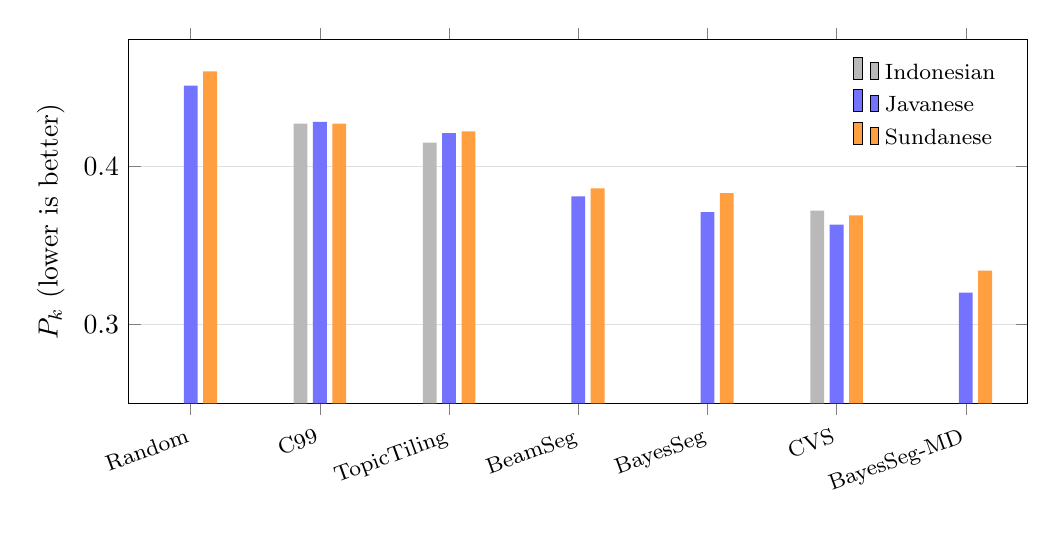
\begin{tikzpicture}
\begin{axis}[
  ybar, bar width=5pt, width=13cm, height=6.2cm,
  ymin=0.25, ymax=0.48, ylabel={$P_k$ (lower is better)},
  symbolic x coords={Random,C99,TopicTiling,BeamSeg,BayesSeg,CVS,BayesSeg-MD},
  xtick={Random,C99,TopicTiling,BeamSeg,BayesSeg,CVS,BayesSeg-MD}, x tick label style={font=\footnotesize, rotate=20, anchor=north east},
  ymajorgrids, grid style={gray!25},
  legend style={at={(0.98,0.97)}, anchor=north east, font=\footnotesize, draw=none},
  legend cell align=left, unbounded coords=jump, enlarge x limits=0.08]
\addplot[fill=gray!55, draw=none] coordinates {
  (Random,nan) (C99,0.427) (TopicTiling,0.415) (BeamSeg,nan) (BayesSeg,nan) (CVS,0.372) (BayesSeg-MD,nan)};
\addplot[fill=blue!55, draw=none] coordinates {
  (Random,0.451) (C99,0.428) (TopicTiling,0.421) (BeamSeg,0.381) (BayesSeg,0.371) (CVS,0.363) (BayesSeg-MD,0.320)};
\addplot[fill=orange!75, draw=none] coordinates {
  (Random,0.460) (C99,0.427) (TopicTiling,0.422) (BeamSeg,0.386) (BayesSeg,0.383) (CVS,0.369) (BayesSeg-MD,0.334)};
\legend{Indonesian, Javanese, Sundanese}
\end{axis}
\end{tikzpicture}
\caption{Segmentation error of the CPU methods with the heading echo removed. All methods beat random boundaries with known $k$; BayesSeg-MD is the most accurate on both regional languages. Encoder and LLM results are added in the final version.\label{fig:pk}}
\end{figure}

% ---------------------------------------------------------------------
%  Table 6. Human evaluation (structure only; no new judgements yet)
% ---------------------------------------------------------------------
\begin{table}[H]
\caption{Human evaluation of summary quality: average rank of the four segmentation strategies (1 = best) over informativeness, coherence and conciseness; 30 articles and three annotators per language. Nemenyi critical difference 0.86 ($\alpha = 0.05$).\label{tab:human}}
\newcolumntype{C}{>{\centering\arraybackslash}X}
\begin{tabularx}{\textwidth}{lCCCC}
\toprule
\textbf{Strategy} & \textbf{Indonesian}\boldmath$^{\,\dagger}$ & \textbf{Javanese} & \textbf{Sundanese} & \textbf{Significant Pairs}\\
\midrule
Set A (unsegmented)          & 3.38 & \tbd & \tbd & \tbd\\
Set B (fixed-size, 8 sent.)  & 2.54 & \tbd & \tbd & \tbd\\
Set C (automatic)            & 1.92 & \tbd & \tbd & \tbd\\
Set D (gold)                 & 2.16 & \tbd & \tbd & \tbd\\
\midrule
Kendall's $W$                & 0.547 & \tbd & \tbd & \\
\bottomrule
\end{tabularx}
\noindent{\footnotesize{$^{\dagger}$ From the conference study (BRIO summarizer); C and D differ significantly from A ($p < 0.001$).}}
\end{table}

% ---------------------------------------------------------------------
%  Figure 3. Critical-difference diagram
%  Generated from the real annotations by:
%    python scripts/human_eval.py analyze --key human_eval/<lang>/key.csv \
%        --sheets "human_eval/<lang>/filled_*.csv" --out human_eval/<lang>/analysis
%  then include the PNG:
% ---------------------------------------------------------------------
% \begin{figure}[H]
% \centering
% \includegraphics[width=12cm]{human_eval/jv/analysis/cd_diagram.png}
% \caption{Critical-difference diagram of summary quality in Javanese (Nemenyi test, $\alpha = 0.05$). Strategies joined by a bar do not differ significantly.\label{fig:cd}}
% \end{figure}

% ---------------------------------------------------------------------
%  Abbreviations (MDPI back-matter macro)
% ---------------------------------------------------------------------
\abbreviations{Abbreviations}{
The following abbreviations are used in this manuscript:\\

\noindent
\begin{tabular}{@{}ll}
CVS    & Content Vector Segmentation\\
LDA    & Latent Dirichlet Allocation\\
LLM    & Large Language Model\\
MDL    & Minimum Description Length\\
NLP    & Natural Language Processing\\
$P_k$  & Probabilistic segmentation error (Beeferman et al.)\\
TF--IDF & Term Frequency--Inverse Document Frequency\\
WD     & WindowDiff
\end{tabular}
}
